\section{Physical Scheduler Evaluation and Strengthening Controls}
\subsection{Primary Campaign and Independent Reconstruction}
The primary campaign contains ten matched blocks on the same Pi 4B 8 GB. Each block evaluates Static-MedRF, CFSM, Tabular-Q, and DQN on one identical 50,000-row held-out trace, for forty 500-second method runs. Method order is randomized within each block and retained in the schedule. A separate 120-second validation-derived round-robin pilot is excluded from formal statistics. Four models remain resident, the recorded governor is \texttt{ondemand}, USB-input power is sampled at 1 Hz using KM003C, and Pi decisions, probabilities, timing, and temperature are logged for every window.

Independent reconstruction finds all forty archived formal runs complete, with 501 power observations and 500 decision--outcome pairs per run: 20,040 raw power frames, 20,000 windows, and 2,000,000 replayed predictions. Raw-frame decoding, sample-time trapezoidal integration, confusion counts, and selected-model predictions agree with the archived summaries. The reconstructed frozen policies reproduce the logged actions from the recorded decision-available state. These checks verify the supplied record; they are not a new physical execution or an independent instrument calibration.

For outcome $z$, the primary effect is the trace-matched difference
\begin{equation}
 d_{b,m}=z_{b,m}-z_{b,\mathrm{Static\mbox{-}MedRF}}.
\end{equation}
Means and two-sided 95\% Student-$t$ intervals are calculated across the ten block differences with nine degrees of freedom~\cite{NISTPaired}. The block, not the 500 within-run windows, is the repeat unit. These intervals do not include meter calibration uncertainty or between-board variability.

The effect size is operationally small. The 13.068 J Tabular-Q saving relative to Static-MedRF over a 500-second run is 1.08\%, equivalent to 26.1 mW average; if that gap persisted continuously, the arithmetic scale would be about 0.23 kWh/year, not an annual field measurement. In the same replay, mean missed-positive presentations rise from 57.8 to 565.9 (about 9.8$\times$). At 100 rows/s, the static 100-row batch profiles (1.544 ms LightLR; 30.953 ms MedRF) imply inference-only duty factors of roughly 0.15\% and 3.10\%, and simple service capacities near 64.7k and 3.23k rows/s. These are scaling diagnostics, not end-to-end throughput benchmarks, but they explain why whole-device power is a low-signal endpoint at the primary low-duty load.

\begin{table*}[t]
\centering\small
\caption{Primary physical results: arithmetic means across ten matched trace blocks per method. Recall and FPR are percentages. Latency is 100-row classifier inference only and excludes scheduler decision time.}
\label{tab:dynamic}
\setlength{\tabcolsep}{5pt}
\begin{tabular}{lrrrrrrrr}\toprule
Method & Energy (J) & Power (W) & F1 & Recall (\%) & FPR (\%) & BA & Mean (ms) & p95 (ms)\\\midrule
\tableinput{tables/dynamic_physical_rows}
\bottomrule\end{tabular}
\end{table*}

\begin{table*}[t]
\centering\small
\caption{Primary paired effects against Static-MedRF, $n=10$ blocks. Positive energy saving means less energy; negative detection differences mean lower scores. Intervals are Student-$t$ 95\% intervals. ``pp'' denotes percentage points.}
\label{tab:paired}
\begin{tabular}{llrll}\toprule
Method & Energy saved (J), 95\% CI & Saved (\%) & $\Delta$F1 (pp), 95\% CI & $\Delta$Recall (pp)\\\midrule
\tableinput{tables/dynamic_paired_rows}
\bottomrule\end{tabular}
\end{table*}

\subsection{Primary Energy--Detection Trade-off and Realized Actions}
Static-MedRF has mean F1 \RFFOne{} and recall \RFRecallPct{}\%. Tabular-Q saves \TQSavingJ{} J (95\% CI \TQSavingJLow{}--\TQSavingJHigh{} J), while DQN saves \DQSavingJ{} J (\DQSavingJLow{}--\DQSavingJHigh{} J). Both have F1 \TQFOne{} and recall \TQRecallPct{}\%. Their reduced FPR does not imply unchanged security performance: the mean missed-positive count rises from \RFFN{} to \TQFN{} per 50,000-row trace, while false positives fall from \RFFP{} to \TQFP{}. No acceptable-loss margin was specified, so the results are not described as equivalent or noninferior detection.

CFSM saves \CFSavingJ{} J but produces F1 \CFFOne{} and FPR \CFFPRPct{}\%. Its unfavorable result is retained without post-test retuning. More importantly, each learned policy selects LightLR in all 5,000 formal windows. The true number of between-window model changes is zero for Tabular-Q and DQN; the source switch counter includes only the initialization transition into the selected detector. The five replay phases therefore change aggregate class-mixture metrics but do not induce learned escalation.

\begin{figure}[t]
\centering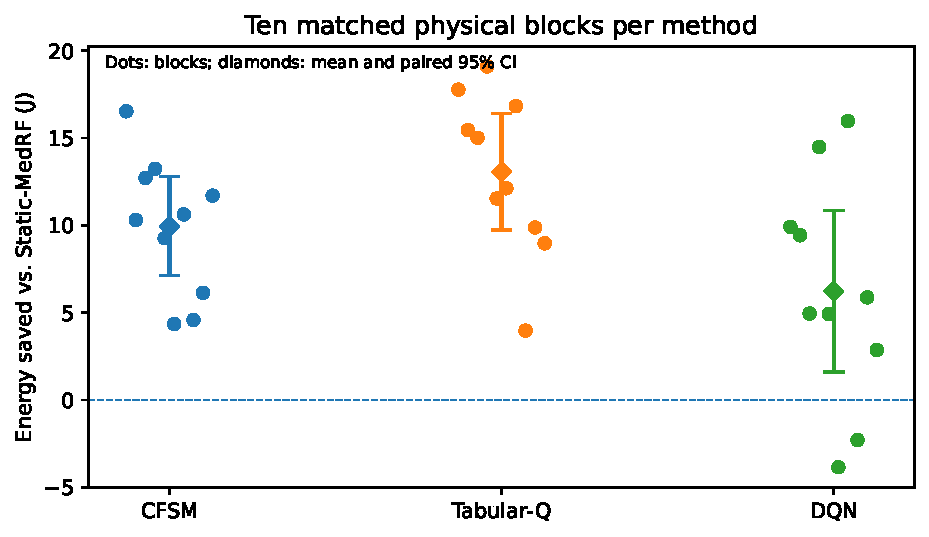
\includegraphics[width=\columnwidth]{figures/paired_energy_savings.pdf}
\caption{Primary blockwise energy saving relative to Static-MedRF. The points are ten physical paired effects per method; positive values denote lower energy.}
\label{fig:energy}
\end{figure}

\subsection{Realized State Support and Phase Behavior}
The primary learned-policy executions reach only four of 324 encoded states. Temperature, queue, and scheduled load remain in one bin; variation is therefore confined to lagged threat context and initialization/previous action. The exact primary four-state IDs are not reconstructed post hoc because the later scheduler-overhead observed-support artifact contains eight states and supplies no unique subset rule---the same ambiguity that caused controller-only power arm to stop. What is auditable is the coverage and full greedy map: Tabular-Q assigns 314/324 states to TinyDT and 10 to LightLR, while DQN assigns all 324 to LightLR; all four states reached in the primary learned-policy runs select LightLR. Because zero-initialized unvisited tabular rows can be governed by deterministic tie behavior, the 314 TinyDT assignments are an off-support safety concern rather than learned evidence.

\begin{table}[t]
\centering\footnotesize
\caption{Primary policy support and full greedy action maps. ``Reached'' is the number of encoded states observed in formal learned-policy execution.}
\label{tab:statesupport}
\setlength{\tabcolsep}{3.2pt}
\begin{tabular}{lrrrr}\toprule
Policy & States & Reached & TinyDT map & LightLR map\\\midrule
Tabular-Q & 324 & 4 & 314 & 10\\
DQN & 324 & 4 & 0 & 324\\
\bottomrule\end{tabular}
\end{table}

\begin{figure}[t]
\centering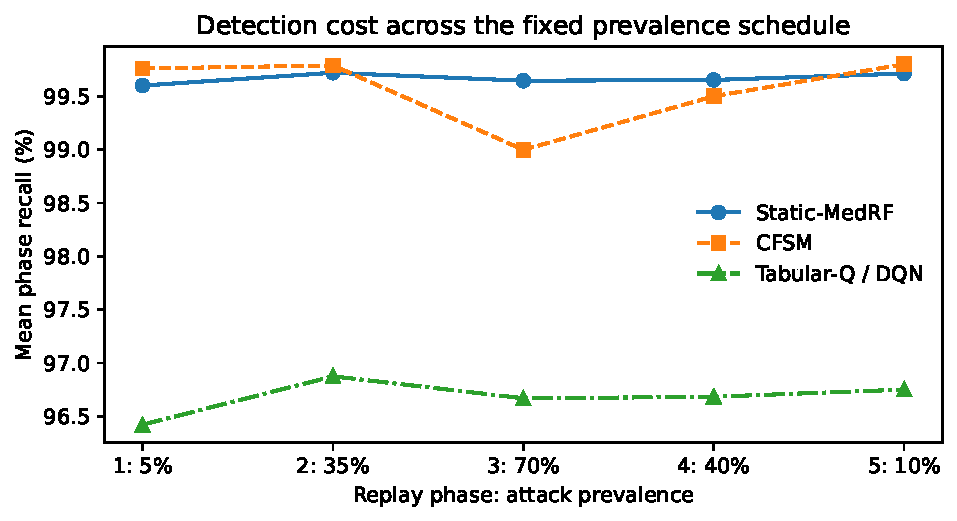
\includegraphics[width=\columnwidth]{figures/phase_recall.pdf}
\caption{Mean recall across the five controlled prevalence phases. Tabular-Q and DQN coincide because both execute LightLR throughout; phase-varying detection therefore reflects a fixed operating point rather than learned phase switching.}
\label{fig:phaserecall}
\end{figure}

\subsection{Matched Static-LightLR Physical Control}
Because both learned policies realize a constant LightLR schedule, we subsequently executed a separate matched control rather than treating the earlier static calibration as equivalent. The matched-control campaign contains ten new trace-matched blocks with Static-LightLR, Tabular-Q, DQN, and Static-MedRF. Forty runs are valid. Two invalid attempts are retained: one DQN preparation failure before workload execution and one interrupted Static-MedRF run that is linked to a single authorized replacement with a new run identifier.

Table~\ref{tab:p1a} gives the critical decomposition. Tabular-Q and Static-LightLR have identical selected-probability hashes, confusion counts, F1, recall, FPR, and balanced accuracy within every block. Their whole-device energy difference is +0.455 J for Tabular-Q with a 95\% paired interval of $[-1.861,2.772]$ J; an exact sign-flip diagnostic gives $p=0.664$. Thus this supplementary campaign does not resolve a directional energy difference between Tabular-Q and direct LightLR deployment. It does not establish statistical equivalence because no equivalence margin was predeclared.

DQN likewise reproduces Static-LightLR detection exactly but consumes +4.525 J more energy on average (95\% CI 2.693--6.357 J; exact sign-flip $p=0.00195$). Static-MedRF consumes +12.471 J more than Static-LightLR while improving F1 by 1.343 percentage points and recall by 2.954 pp; its FPR is also 0.174 pp higher. This matched control therefore separates the primary Static-MedRF contrast into detector choice and controller/runtime effects: the supplementary campaign resolves no directional whole-device energy difference between Tabular-Q and direct LightLR at this resolution, whereas DQN has an additional measured whole-device premium under an identical detector schedule.

\begin{table*}[t]
\centering\small
\caption{Supplementary paired contrasts against Static-LightLR, $n=10$ blocks. Energy and power are first method minus Static-LightLR; detection differences are percentage points. This matched control is post-hoc strengthening evidence and does not replace the primary campaign.}
\label{tab:p1a}
\setlength{\tabcolsep}{4.3pt}
\begin{tabular}{lrrrrr}\toprule
Method & $\Delta E$ (J), 95\% CI & $\Delta P$ (mW), 95\% CI & $\Delta$F1 & $\Delta$Recall & $\Delta$FPR\\\midrule
\tableinput{tables/p1a_static_lightlr_rows}
\bottomrule\end{tabular}
\end{table*}


\subsection{Isolated Scheduler Decision Overhead}
The corrected scheduler-overhead benchmark measures only the boundary from an already encoded scheduler state to the selected action. The original 240-unit attempt is retained as invalid because the final validator identified a fixed-MedRF substitution in the CFSM path and missing telemetry. One authorized corrected replacement repeats the frozen design; 240/240 corrected units pass, and a 5,000-state CFSM comparison reports zero semantic mismatches.

On the observed state support, mean state-to-action time is 0.739~$\mu$s for the trivial Static-LightLR selector, 6.582~$\mu$s for CFSM, 10.796~$\mu$s for Tabular-Q, and 1.567 ms for DQN (Table~\ref{tab:p1b}). The corresponding DQN mean is about 145 times Tabular-Q, but still only 0.157\% of the one-second scheduling interval. The exhaustive 324-state stream yields the same ordering and is reported in the supplement. These timing measurements are kept separate from classifier inference and cannot be converted directly into joules; they therefore support a computation-overhead comparison but do not by themselves explain the DQN energy premium in the matched-control campaign.

\begin{table}[t]
\centering\footnotesize
\caption{Corrected state-to-action timing on observed held-out support; 30 paired benchmark blocks per method. The CI is across block means.}
\label{tab:p1b}
\setlength{\tabcolsep}{3.2pt}
\begin{tabular}{lrrrr}\toprule
Method & Mean ($\mu$s) & 95\% CI ($\mu$s) & p95 ($\mu$s) & \% of 1 s\\\midrule
\tableinput{tables/p1b_overhead_rows}
\bottomrule\end{tabular}
\end{table}

\subsection{Support-Limited Policy Robustness and Sensitivity}
The post-hoc software analyses ask whether the LightLR collapse is tied to one policy seed or one nearby specification. Ten new Tabular-Q seeds and ten new DQN seeds all select LightLR on 100\% of held-out windows; for each algorithm the observed-support collapse frequency is 10/10 (Wilson 95\% interval 0.722--1.000). This statement is deliberately support-limited. Greedy action maps over all 324 encoded states vary across seeds, especially for DQN, so the result is not a claim of global policy-map stability.

The reward/state sensitivity study contains 85 valid runs and every held-out policy is single-action. Eighty select LightLR; the five exceptions are the Tabular-Q detection-only reward, which selects MedRF throughout and recovers the Static-MedRF detection operating point. All thirty Tabular-Q state-ablation runs select LightLR. The hyperparameter sensitivity study adds 35 valid Tabular-Q $\alpha/\gamma$ sensitivity runs, and all 35 select LightLR on held-out support. Table~\ref{tab:p1robust} summarizes these results. The sweeps therefore support a narrow mechanism: the observed support strongly favors one static operating point across seeds, state removals, and the predefined $\alpha/\gamma$ range, while changing the objective to detection-only changes \emph{which} static detector is selected. None of these post-hoc policies replaces the frozen primary policy.

\begin{table*}[t]
\centering\small
\caption{Post-hoc policy robustness on held-out support. ``Single'' means one detector is selected throughout each evaluated trace after initialization. Raw source switch counts include initialization; between-window switching is zero for the listed collapsed policies.}
\label{tab:p1robust}
\begin{tabular}{lrrrl}\toprule
Analysis & Runs & Held-out detector outcome & Single & Boundary\\\midrule
\tableinput{tables/p1_robustness_rows}
\bottomrule\end{tabular}
\end{table*}

\subsection{Temperature and Order Diagnostics}
Post-inference temperatures remain low across the primary physical workload and no throttle event is logged. Temperature, queue, and scheduled arrival-rate bins occupy only one bin each, limiting evidence for thermal or congestion adaptation. The supplementary matched-control temperature contrasts against Static-LightLR also have intervals crossing zero for both learned policies. These observations do not establish high-temperature safety or resource-state generality.

The original primary randomization is not a balanced Latin square. A retained post-hoc block/position analysis and leave-one-block-out/sign-flip diagnostics preserve the direction of the primary energy contrasts, but they cannot remove unmeasured ambient drift. The matched-control campaign uses a separately frozen order and is interpreted only within that supplementary campaign.
